% document
\documentclass[10pt,graphics,aspectratio=169,table]{beamer}
\usepackage{../code}
\usepackage{csquotes}
\usepackage{hyperref}
\usepackage{tikz}
\usepackage{pgfplots}
% theme
\usetikzlibrary{arrows}
\tikzstyle{line}=[draw] % here
\usetikzlibrary{decorations.pathmorphing}
\tikzset{arrow/.style={-latex, shorten >=.5ex, shorten <=.5ex}}

\usetheme{metropolis}
% packages
\title{Lesson 5}
\author{Christian Schwarz, Jakob Krebs}
\date{25.11.2019}
\begin{document}
\maketitle

\begin{frame}{Contents}
    \tableofcontents
\end{frame}


\section{Source Code and Solutions}
\begin{frame}{Sources and Solutions}
    \begin{itemize}
        \item we publish all code written in this course at \url{https://github.com/jkrbs/c_lessons}
        \item we will publish example solutions of the tasks on same site
        \item send us questions or your solutions to c-lessons@deutschland.gmbh
    \end{itemize}
\end{frame}

\section{Typedef}
\begin{frame}[fragile]{typedefs}
    In previous lessons we said that \code{size_t} or \code{bool} are not
    native to the C type system, but library types built upon it.
    But how do you define a type?

    \begin{codeblock}
typedef int foo_t;

// we can now use foo_t just like short:
void foo(){
    foo_t x = 3;
    short y = 4;
    foo_t z = x + y;
}
    \end{codeblock}

    Using typedefs we can abstract away plattform differences,
    shorten long type names (function pointers) etc.
    But don't go out typedef'ing every integer you use :).
\end{frame}

\begin{frame}[fragile]{typedef with structs}
    In many other programming languages,
    (including \code{C++}).
    We can use structs and enums just like the predefined types.
    So why do we have to write \code{struct foo} in \code{C}, instead of just
    \code{foo} ?. Well we don't \textbf{have} to.
    We can typedef our struct definition to be it's own type:
    \code{typedef struct foo foo;}. And we can combine this with the definition:
    \begin{codeblock}
// struct point is the struct name, can be used as normal
// the struct and typedef name can also be different
typedef struct point{
    int x, y;
}point; //point now means the same as struct point

point add(point p1, point p2){
    point sum = {p1.x + p2.x, p1.y + p2.y};
    return sum;
}
    \end{codeblock}
\end{frame}
    \begin{frame}[fragile]{legacy code with unnamed structs}
    In old code the struct name is also left out:

    \begin{codeblock}
typedef struct{
    //point* p; //this wouldn't work
    int x, y;
}point;
// C++ compilers would complain about a type conflict here
// struct point;
    \end{codeblock}

    This can cause problems in forward declarations and when you
    want to have pointers to the struct
    inside itself, since the typedef isn't available until the end.

    Therefore we don't do that.
\end{frame}

\section{data structures}

\subsection{linked list}
\begin{frame}{linked lists}

	\begin{tikzpicture}[scale=.73,font=\scriptsize]
			
		\draw (-2.5,.1) -- (-1,.1);
		\draw (-2.5,.1) -- (-2.5,.45);
		\draw (-2.5,.45) -- (-1,.45);
		\draw (-1,.45) -- (-1,.1);
		\node[circle, thick, draw=black, minimum size=5pt, inner sep = 0pt] at (-1.18,.275) {};
		\node at (-2.6,.275) [right] {head};
		\draw (-1.05,.275) edge[thick,out=0,in=135,->,shorten >=.2ex] (0,1);
	
		\draw (0,0) -- (0,1);
		\draw (0,0) -- (2,0);
		\draw (0,1) -- (2,1);
		\draw (2,0) -- (2,1);
		
		\draw (.1,.1) -- (.1,.45);
		\draw (.1,.1) -- (1.9,.1);
		\draw (.1,.45) -- (1.9,.45);
		\draw (1.9,.1) -- (1.9,.45);
		\node at (0,.275) [right] {next};
		
		\node[circle, thick, draw=black, minimum size=5pt, inner sep = 0pt] at (1.72,.275) {};
		\begin{uncoverenv}<-3>
			\draw (1.85,.275) edge[thick,out=0,in=135,->,shorten >=.2ex] (3,1);
		\end{uncoverenv}
		\begin{uncoverenv}<4>
			\draw (1.85,.275) edge[red,thick,out=0,in=135,->,shorten >=.2ex] (3,1);
		\end{uncoverenv}
		
		\draw (.1,.55) -- (.1,.9);
		\draw (.1,.55) -- (1.9,.55);
		\draw (.1,.9) -- (1.9,.9);
		\draw (1.9,.55) -- (1.9,.9);
		\node at (0,.725) [right] {value = ...};
		
		
		\draw (3,0) -- (3,1);
		\draw (3,0) -- (5,0);
		\draw (3,1) -- (5,1);
		\draw (5,0) -- (5,1);
		
		\draw (3.1,.1) -- (3.1,.45);
		\draw (3.1,.1) -- (4.9,.1);
		\draw (3.1,.45) -- (4.9,.45);
		\draw (4.9,.1) -- (4.9,.45);
		\node at (3,.275) [right] {next};
		
		\node[circle, thick, draw=black, minimum size=5pt, inner sep = 0pt] at (4.72,.275) {};
		\draw (4.85,.275) edge[thick,out=0,in=135,->,shorten >=.2ex] (6,1);
		
		
		\draw (3.1,.55) -- (3.1,.9);
		\draw (3.1,.55) -- (4.9,.55);
		\draw (3.1,.9) -- (4.9,.9);
		\draw (4.9,.55) -- (4.9,.9);
		\node at (3,.725) [right] {value = ...};
		
		
		\draw (6,0) -- (6,1);
		\draw (6,0) -- (8,0);
		\draw (6,1) -- (8,1);
		\draw (8,0) -- (8,1);
		
		\draw (6.1,.1) -- (6.1,.45);
		\draw (6.1,.1) -- (7.9,.1);
		\draw (6.1,.45) -- (7.9,.45);
		\draw (7.9,.1) -- (7.9,.45);
		\node at (6,.275) [right] {next};
		
		\node[circle, thick, draw=black, minimum size=5pt, inner sep = 0pt] at (7.72,.275) {};
		\draw (7.85,.275) edge[thick,out=0,in=135,->,shorten >=.2ex] (9,1);
		
		\draw (6.1,.55) -- (6.1,.9);
		\draw (6.1,.55) -- (7.9,.55);
		\draw (6.1,.9) -- (7.9,.9);
		\draw (7.9,.55) -- (7.9,.9);
		\node at (6,.725) [right] {value = ...};
		
		
		\draw (9,0) -- (9,1);
		\draw (9,0) -- (11,0);
		\draw (9,1) -- (11,1);
		\draw (11,0) -- (11,1);
		
		\draw (9.1,.1) -- (9.1,.45);
		\draw (9.1,.1) -- (10.9,.1);
		\draw (9.1,.45) -- (10.9,.45);
		\draw (10.9,.1) -- (10.9,.45);
		\node at (9,.275) [right] {next};
		
		
		\node[circle, thick, draw=black, minimum size=5pt, inner sep = 0pt] at (10.72,.275) {};
		\draw (10.85,.275) edge[thick,out=0,in=155,->,shorten >=.2ex] (11.5,.45);
		
		\draw (9.1,.55) -- (9.1,.9);
		\draw (9.1,.55) -- (10.9,.55);
		\draw (9.1,.9) -- (10.9,.9);
		\draw (10.9,.55) -- (10.9,.9);
		\node at (9,.725) [right] {value = ...};

		\draw (11.5,.1) -- (11.5,.45);
		\draw (11.5,.1) -- (12.5,.1);
		\draw (11.5,.45) -- (12.5,.45);
		\draw (12.5,.1) -- (12.5,.45);
		\node at (11.4,.265) [right] {NULL};
		
		
		\begin{uncoverenv}<2->
			\draw (2,-.5) -- (2,-1.5);
			\draw (2,-.5) -- (4,-.5);
			\draw (4,-.5) -- (4,-1.5);
			\draw (4,-1.5) -- (2,-1.5);
			
			\draw (2.1,-.6) -- (2.1, -.95);
			\draw (2.1,-.6) -- (3.9,-.6);
			\draw (3.9,-.6) -- (3.9,-.95);
			\draw (3.9,-.95) -- (2.1,-.95);
			\node at (2,-.775) [right] {value = ...};
			
			
			\draw (2.1, -1.05) -- (2.1, -1.4);
			\draw (2.1,-1.05) -- (3.9,-1.05);
			\draw (3.9,-1.05) -- (3.9,-1.4);
			\draw (3.9,-1.4) -- (2.1,-1.4);
			\node at (2,-1.225) [right] {next};
			\node[circle, thick, draw=black, minimum size=5pt, inner sep = 0pt] at (3.72,-1.225) {};
			
			
		\end{uncoverenv}
		\begin{uncoverenv}<3->
			\draw [thick,blue,->,shorten >=.2ex] (3.85,-1.225) to[out=0,in=-35] (4,-.4) to[out=180-35,in=-45] (2.5,-.1) to[out=180-45,in=135] (3,1);
		\end{uncoverenv}
		\begin{uncoverenv}<5->
			\draw [thick,red,->,shorten >=.2ex] (1.72,.145) to[out=-90,in=135] (2,-.5);
		\end{uncoverenv}
		
		
	\end{tikzpicture}
	\ \\\ \\
	\begin{itemize}[<+->]
		\item Now we can build lists of this structures.
		\item If we want to insert a value at a specific position...
		\item ... we just have to change the pointers.
	\end{itemize}
	
	\begin{itemize}
		\item<6-> Additionally we can easily iterate through this list.
		\item<6-> But only in one direction.
	\end{itemize}
	
\end{frame}

\begin{frame}{Intermediate Task: Linked List Insertion}
    No we will try to implement in code what we just saw.
    You can start out with the code you can find at

    \begin{small}
    \url{https://jkrbs.github.io/c_lessons/tasks/intermediate_5_linked_list_insertion.c}
    \end{small}
    
    Or just click on \code{Lesson 5 Intermediate Task Starting Point: Linked List Insertion}
   
    on our website (\url{https://jkrbs.github.io/c_lessons}).


    Task: Write the function \code{list_insert} and test if your code works!

\end{frame}

\subsection{double linked list}

\begin{frame}{Double-linked lists}

	\begin{tikzpicture}[scale=.73,font=\scriptsize]
			
		\draw (-2.5,.1) -- (-1,.1);
		\draw (-2.5,.1) -- (-2.5,.45);
		\draw (-2.5,.45) -- (-1,.45);
		\draw (-1,.45) -- (-1,.1);
		\node[circle, thick, draw=black, minimum size=5pt, inner sep = 0pt] at (-1.18,.275) {};
		\node at (-2.6,.275) [right] {head};
		\draw (-1.05,.275) edge[thick,out=0,in=135,->,shorten >=.2ex] (0,1);
		
		\draw (-2,-.1) -- (-1,-.1);
		\draw (-2,-.1) -- (-2,-.45);
		\draw (-2,-.45) -- (-1,-.45);
		\draw (-1,-.45) -- (-1,-.1);
		\node at (-2.1,-.275) [right] {NULL};
	
		\draw (0,-.45) -- (0,1);
		\draw (0,-.45) -- (2,-.45);
		\draw (0,1) -- (2,1);
		\draw (2,-.45) -- (2,1);
		
		\draw (.1,-.35) -- (.1,0);
		\draw (.1,-.35) -- (1.9,-.35);
		\draw (.1,0) -- (1.9,0);
		\draw (1.9,-.35) -- (1.9,0);
		\node at (.3,-.225) [right] {prev};
		
		\node[circle, thick, draw=black, minimum size=5pt, inner sep = 0pt] at (.28,-.175) {};
		\draw (.15,-.175) edge[thick,out=180,in=-35,->,shorten >=.2ex] (-1,-.45);
		
		\draw (.1,.1) -- (.1,.45);
		\draw (.1,.1) -- (1.9,.1);
		\draw (.1,.45) -- (1.9,.45);
		\draw (1.9,.1) -- (1.9,.45);
		\node at (0,.275) [right] {next};
		
		\node[circle, thick, draw=black, minimum size=5pt, inner sep = 0pt] at (1.72,.275) {};
		\begin{uncoverenv}<-3>
			\draw (1.85,.275) edge[thick,out=0,in=135,->,shorten >=.2ex] (3,1);
		\end{uncoverenv}
		\begin{uncoverenv}<4>
			\draw (1.85,.275) edge[red,thick,out=0,in=135,->,shorten >=.2ex] (3,1);
		\end{uncoverenv}
		
		\draw (.1,.55) -- (.1,.9);
		\draw (.1,.55) -- (1.9,.55);
		\draw (.1,.9) -- (1.9,.9);
		\draw (1.9,.55) -- (1.9,.9);
		\node at (0,.725) [right] {value = ...};
		
		
		\draw (3,-.45) -- (3,1);
		\draw (3,-.45) -- (5,-.45);
		\draw (3,1) -- (5,1);
		\draw (5,-.45) -- (5,1);
		
		\draw (3.1,-.35) -- (3.1,0);
		\draw (3.1,-.35) -- (4.9,-.35);
		\draw (3.1,0) -- (4.9,0);
		\draw (4.9,-.35) -- (4.9,0);
		\node at (3.3,-.225) [right] {prev};
		
		\node[circle, thick, draw=black, minimum size=5pt, inner sep = 0pt] at (3.28,-.175) {};
		\begin{uncoverenv}<-3>
			\draw (3.15,-.175) edge[thick,out=180,in=-45,->,shorten >=.2ex] (2,-.45);
		\end{uncoverenv}
		\begin{uncoverenv}<4>
			\draw (3.15,-.175) edge[red,thick,out=180,in=-45,->,shorten >=.2ex] (2,-.45);
		\end{uncoverenv}
		
		\draw (3.1,.1) -- (3.1,.45);
		\draw (3.1,.1) -- (4.9,.1);
		\draw (3.1,.45) -- (4.9,.45);
		\draw (4.9,.1) -- (4.9,.45);
		\node at (3,.275) [right] {next};
		
		\node[circle, thick, draw=black, minimum size=5pt, inner sep = 0pt] at (4.72,.275) {};
		\draw (4.85,.275) edge[thick,out=0,in=135,->,shorten >=.2ex] (6,1);
		
		
		\draw (3.1,.55) -- (3.1,.9);
		\draw (3.1,.55) -- (4.9,.55);
		\draw (3.1,.9) -- (4.9,.9);
		\draw (4.9,.55) -- (4.9,.9);
		\node at (3,.725) [right] {value = ...};
		
		
		\draw (6,-.45) -- (6,1);
		\draw (6,-.45) -- (8,-.45);
		\draw (6,1) -- (8,1);
		\draw (8,-.45) -- (8,1);
		
		\draw (6.1,-.35) -- (6.1,0);
		\draw (6.1,-.35) -- (7.9,-.35);
		\draw (6.1,0) -- (7.9,0);
		\draw (7.9,-.35) -- (7.9,0);
		\node at (6.3,-.225) [right] {prev};
		
		\node[circle, thick, draw=black, minimum size=5pt, inner sep = 0pt] at (6.28,-.175) {};
		\draw (6.15,-.175) edge[thick,out=180,in=-45,->,shorten >=.2ex] (5,-.45);
		
		\draw (6.1,.1) -- (6.1,.45);
		\draw (6.1,.1) -- (7.9,.1);
		\draw (6.1,.45) -- (7.9,.45);
		\draw (7.9,.1) -- (7.9,.45);
		\node at (6,.275) [right] {next};
		
		\node[circle, thick, draw=black, minimum size=5pt, inner sep = 0pt] at (7.72,.275) {};
		\draw (7.85,.275) edge[thick,out=0,in=135,->,shorten >=.2ex] (9,1);
		
		\draw (6.1,.55) -- (6.1,.9);
		\draw (6.1,.55) -- (7.9,.55);
		\draw (6.1,.9) -- (7.9,.9);
		\draw (7.9,.55) -- (7.9,.9);
		\node at (6,.725) [right] {value = ...};
		
		
		\draw (9,-.45) -- (9,1);
		\draw (9,-.45) -- (11,-.45);
		\draw (9,1) -- (11,1);
		\draw (11,-.45) -- (11,1);
		
		\draw (9.1,-.35) -- (9.1,0);
		\draw (9.1,-.35) -- (10.9,-.35);
		\draw (9.1,0) -- (10.9,0);
		\draw (10.9,-.35) -- (10.9,0);
		\node at (9.3,-.225) [right] {prev};
		
		\node[circle, thick, draw=black, minimum size=5pt, inner sep = 0pt] at (9.28,-.175) {};
		\draw (9.15,-.175) edge[thick,out=180,in=-45,->,shorten >=.2ex] (8,-.45);
		
		\draw (9.1,.1) -- (9.1,.45);
		\draw (9.1,.1) -- (10.9,.1);
		\draw (9.1,.45) -- (10.9,.45);
		\draw (10.9,.1) -- (10.9,.45);
		\node at (9,.275) [right] {next};
		
		
		\node[circle, thick, draw=black, minimum size=5pt, inner sep = 0pt] at (10.72,.275) {};
		\draw (10.85,.275) edge[thick,out=0,in=155,->,shorten >=.2ex] (11.5,.45);
		
		\draw (9.1,.55) -- (9.1,.9);
		\draw (9.1,.55) -- (10.9,.55);
		\draw (9.1,.9) -- (10.9,.9);
		\draw (10.9,.55) -- (10.9,.9);
		\node at (9,.725) [right] {value = ...};

		\draw (11.5,.1) -- (11.5,.45);
		\draw (11.5,.1) -- (12.5,.1);
		\draw (11.5,.45) -- (12.5,.45);
		\draw (12.5,.1) -- (12.5,.45);
		\node at (11.4,.265) [right] {NULL};
		
		
		\begin{uncoverenv}<2->
			\draw (2,-1.5) -- (2,-2.95);
			\draw (2,-1.5) -- (4,-1.5);
			\draw (4,-1.5) -- (4,-2.95);
			\draw (4,-2.95) -- (2,-2.95);
			
			\draw (2.1,-1.6) -- (2.1, -1.95);
			\draw (2.1,-1.6) -- (3.9,-1.6);
			\draw (3.9,-1.6) -- (3.9,-1.95);
			\draw (3.9,-1.95) -- (2.1,-1.95);
			\node at (2,-1.775) [right] {value = ...};
			
			\draw (2.1, -2.05) -- (2.1, -2.4);
			\draw (2.1,-2.05) -- (3.9,-2.05);
			\draw (3.9,-2.05) -- (3.9,-2.4);
			\draw (3.9,-2.4) -- (2.1,-2.4);
			\node at (2,-2.225) [right] {next};
			\node[circle, thick, draw=black, minimum size=5pt, inner sep = 0pt] at (3.72,-2.225) {};
			
			\draw (2.1, -2.5) -- (2.1, -2.85);
			\draw (2.1,-2.5) -- (3.9,-2.5);
			\draw (3.9,-2.5) -- (3.9,-2.85);
			\draw (3.9,-2.85) -- (2.1,-2.85);
			\node at (2.3,-2.725) [right] {prev};
			\node[circle, thick, draw=black, minimum size=5pt, inner sep = 0pt] at (2.28,-2.675) {};
			
			
		\end{uncoverenv}
		\begin{uncoverenv}<3->
			\draw [thick,blue,->,shorten >=.2ex] (3.85,-2.225) to[out=0,in=-35] (4,-1.4) to[out=180-35,in=-45] (2.8,-1.1) to[out=180-45,in=135] (3,1);
			\draw [thick,blue,->,shorten >=.2ex] (2.15,-2.675) to[out=180,in=180+35] (1.8,-1) to[out=35,in=-45] (2,-.45);
		\end{uncoverenv}
		\begin{uncoverenv}<5>
			\draw [thick,red,->,shorten >=.2ex] (1.85,.275) to[out=0,in=90] (2.25,-.5) to[out=270,in=135] (2,-1.5);
			\draw [thick,red,->,shorten >=.2ex] (3.28,-.305) to[out=-90,in=90] (4.6,-1.8) to[out=270,in=-45] (4,-2.95);
		\end{uncoverenv}
		
		
	\end{tikzpicture}

	\begin{itemize}[<+->]
		\item With a pointer in each direction, we can iterate forwards and backwards.
		\item When inserting a value we now have to change a little more.
	\end{itemize}
\end{frame}
\subsection{tree}
\begin{frame}{Binary trees}
	\begin{columns}[T]
		\column{.5\textwidth}
		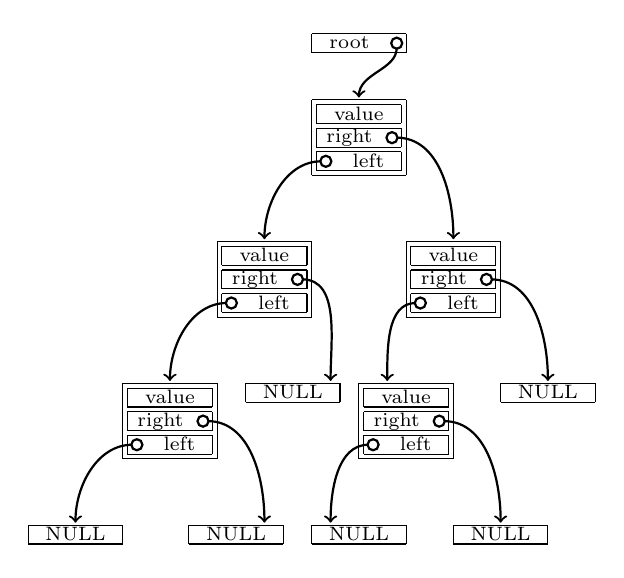
\begin{tikzpicture}[scale=.12,font=\scriptsize]
			\draw (-5,0) -- (5,0);
			\draw (5,0) -- (5,-2);
			\draw (5,-2) -- (-5,-2);
			\draw (-5,-2) -- (-5,0);
			
			\node at (-1,.7)[below] {root};
			\node[circle, thick, draw=black, minimum size=4pt, inner sep = 0pt] at (4,-1) {};
			\draw [thick,->,shorten >=.2ex,shorten <=.4ex] (4,-1) to[out=-90,in=90] (0,-7);
			
			
			\draw (-5,-7) -- (5,-7);
			\draw (5,-7) -- (5,-15);
			\draw (5,-15) -- (-5,-15);
			\draw (-5,-15) -- (-5,-7);
			
			\draw (-4.5,-7.5) -- (4.5,-7.5);
			\draw (4.5,-7.5) -- (4.5,-9.5);
			\draw (4.5,-9.5) -- (-4.5,-9.5);
			\draw (-4.5,-9.5) -- (-4.5,-7.5);
			\node at (0,-6.7)[below] {value};
			
			\draw (-4.5,-10) -- (4.5,-10);
			\draw (4.5,-10) -- (4.5,-12);
			\draw (4.5,-12) -- (-4.5,-12);
			\draw (-4.5,-12) -- (-4.5,-10);
			\node at (-1,-9.1)[below] {right};
			\node[circle, thick, draw=black, minimum size=4pt, inner sep = 0pt] at (3.5,-11) {};
			\draw [thick,->,shorten >=.2ex,shorten <=.4ex] (3.5,-11) to[out=0,in=90] (10,-22);
			
			\draw (-4.5,-12.5) -- (4.5,-12.5);
			\draw (4.5,-12.5) -- (4.5,-14.5);
			\draw (4.5,-14.5) -- (-4.5,-14.5);
			\draw (-4.5,-14.5) -- (-4.5,-12.5);
			\node at (1,-11.7)[below] {left};
			\node[circle, thick, draw=black, minimum size=4pt, inner sep = 0pt] at (-3.5,-13.5) {};
			\draw [thick,->,shorten >=.2ex,shorten <=.4ex] (-3.5,-13.5) to[out=-180,in=90] (-10,-22);
			
			
			\draw (-15,-22) -- (-5,-22);
			\draw (-5,-22) -- (-5,-30);
			\draw (-5,-30) -- (-15,-30);
			\draw (-15,-30) -- (-15,-22);
			
			\draw (-14.5,-22.5) -- (-5.5,-22.5);
			\draw (-5.5,-22.5) -- (-5.5,-24.5);
			\draw (-5.5,-24.5) -- (-14.5,-24.5);
			\draw (-14.5,-24.5) -- (-14.5,-22.5);
			\node at (-10,-21.7)[below] {value};
			
			\draw (-14.5,-25) -- (-5.5,-25);
			\draw (-5.5,-25) -- (-5.5,-27);
			\draw (-5.5,-27) -- (-14.5,-27);
			\draw (-14.5,-27) -- (-14.5,-25);
			\node at (-11,-24.1)[below] {right};
			\node[circle, thick, draw=black, minimum size=4pt, inner sep = 0pt] at (-6.5,-26) {};
			\draw [thick,->,shorten >=.2ex,shorten <=.4ex] (-6.5,-26) to[out=0,in=90] (-3,-37);
			
			\draw (-14.5,-27.5) -- (-5.5,-27.5);
			\draw (-5.5,-27.5) -- (-5.5,-29.5);
			\draw (-5.5,-29.5) -- (-14.5,-29.5);
			\draw (-14.5,-29.5) -- (-14.5,-27.5);
			\node at (-9,-26.7)[below] {left};
			\node[circle, thick, draw=black, minimum size=4pt, inner sep = 0pt] at (-13.5,-28.5) {};
			\draw [thick,->,shorten >=.2ex,shorten <=.4ex] (-13.5,-28.5) to[out=180,in=90] (-20,-37);
			
			
			
			\draw (5,-22) -- (15,-22);
			\draw (15,-22) -- (15,-30);
			\draw (15,-30) -- (5,-30);
			\draw (5,-30) -- (5,-22);
			
			\draw (5.5,-22.5) -- (14.5,-22.5);
			\draw (14.5,-22.5) -- (14.5,-24.5);
			\draw (14.5,-24.5) -- (5.5,-24.5);
			\draw (5.5,-24.5) -- (5.5,-22.5);
			\node at (10,-21.7)[below] {value};
			
			\draw (5.5,-25) -- (14.5,-25);
			\draw (14.5,-25) -- (14.5,-27);
			\draw (14.5,-27) -- (5.5,-27);
			\draw (5.5,-27) -- (5.5,-25);
			\node at (9,-24.1)[below] {right};
			\node[circle, thick, draw=black, minimum size=4pt, inner sep = 0pt] at (13.5,-26) {};
			\draw [thick,->,shorten >=.2ex,shorten <=.4ex] (13.5,-26) to[out=0,in=90] (20,-37);
			
			\draw (5.5,-27.5) -- (14.5,-27.5);
			\draw (14.5,-27.5) -- (14.5,-29.5);
			\draw (14.5,-29.5) -- (5.5,-29.5);
			\draw (5.5,-29.5) -- (5.5,-27.5);
			\node at (11,-26.7)[below] {left};
			\node[circle, thick, draw=black, minimum size=4pt, inner sep = 0pt] at (6.5,-28.5) {};
			\draw [thick,->,shorten >=.2ex,shorten <=.4ex] (6.5,-28.5) to[out=180,in=90] (3,-37);
			
			
			
			
			\draw (-25,-37) -- (-15,-37);
			\draw (-15,-37) -- (-15,-45);
			\draw (-15,-45) -- (-25,-45);
			\draw (-25,-45) -- (-25,-37);
			
			\draw (-24.5,-37.5) -- (-15.5,-37.5);
			\draw (-15.5,-37.5) -- (-15.5,-39.5);
			\draw (-15.5,-39.5) -- (-24.5,-39.5);
			\draw (-24.5,-39.5) -- (-24.5,-37.5);
			\node at (-20,-36.7)[below] {value};
			
			\draw (-24.5,-40) -- (-15.5,-40);
			\draw (-15.5,-40) -- (-15.5,-42);
			\draw (-15.5,-42) -- (-24.5,-42);
			\draw (-24.5,-42) -- (-24.5,-40);
			\node at (-21,-39.1)[below] {right};
			\node[circle, thick, draw=black, minimum size=4pt, inner sep = 0pt] at (-16.5,-41) {};
			\draw [thick,->,shorten >=.2ex,shorten <=.4ex] (-16.5,-41) to[out=0,in=90] (-10,-52);
			
			\draw (-24.5,-42.5) -- (-15.5,-42.5);
			\draw (-15.5,-42.5) -- (-15.5,-44.5);
			\draw (-15.5,-44.5) -- (-24.5,-44.5);
			\draw (-24.5,-44.5) -- (-24.5,-42.5);
			\node at (-19,-41.7)[below] {left};
			\node[circle, thick, draw=black, minimum size=4pt, inner sep = 0pt] at (-23.5,-43.5) {};
			\draw [thick,->,shorten >=.2ex,shorten <=.4ex] (-23.5,-43.5) to[out=-180,in=90] (-30,-52);
	
	
	
	
			\draw (0,-37) -- (10,-37);
			\draw (10,-37) -- (10,-45);
			\draw (10,-45) -- (0,-45);
			\draw (0,-45) -- (0,-37);
			
			\draw (.5,-37.5) -- (9.5,-37.5);
			\draw (9.5,-37.5) -- (9.5,-39.5);
			\draw (9.5,-39.5) -- (.5,-39.5);
			\draw (.5,-39.5) -- (.5,-37.5);
			\node at (5,-36.7)[below] {value};
			
			\draw (.5,-40) -- (9.5,-40);
			\draw (9.5,-40) -- (9.5,-42);
			\draw (9.5,-42) -- (.5,-42);
			\draw (.5,-42) -- (.5,-40);
			\node at (4,-39.1)[below] {right};
			\node[circle, thick, draw=black, minimum size=4pt, inner sep = 0pt] at (8.5,-41) {};
			\draw [thick,->,shorten >=.2ex,shorten <=.4ex] (8.5,-41) to[out=0,in=90] (15,-52);
			
			\draw (.5,-42.5) -- (9.5,-42.5);
			\draw (9.5,-42.5) -- (9.5,-44.5);
			\draw (9.5,-44.5) -- (.5,-44.5);
			\draw (.5,-44.5) -- (.5,-42.5);
			\node at (6,-41.7)[below] {left};
			\node[circle, thick, draw=black, minimum size=4pt, inner sep = 0pt] at (1.5,-43.5) {};
			\draw [thick,->,shorten >=.2ex,shorten <=.4ex] (1.5,-43.5) to[out=-180,in=90] (-3,-52);
	
	
	
			\draw (-35,-52) -- (-25,-52);
			\draw (-35,-52) -- (-35,-54);
			\draw (-25,-52) -- (-25,-54);
			\draw (-35,-54) -- (-25,-54);
			\node at (-30,-51.2)[below] {NULL};
	
	
	
	
			\draw (-18,-52) -- (-8,-52);
			\draw (-18,-52) -- (-18,-54);
			\draw (-8,-52) -- (-8,-54);
			\draw (-18,-54) -- (-8,-54);
			\node at (-13,-51.2)[below] {NULL};
	
	
	
	
			\draw (-5,-52) -- (5,-52);
			\draw (-5,-52) -- (-5,-54);
			\draw (5,-52) -- (5,-54);
			\draw (-5,-54) -- (5,-54);
			\node at (0,-51.2)[below] {NULL};
	
	
	
	
			\draw (10,-52) -- (20,-52);
			\draw (20,-52) -- (20,-54);
			\draw (10,-52) -- (10,-54);
			\draw (10,-54) -- (20,-54);
			\node at (15,-51.2)[below] {NULL};
	
	
	
			\draw (-12,-37) -- (-2,-37);
			\draw (-12,-37) -- (-12,-39);
			\draw (-2,-37) -- (-2,-39);
			\draw (-12,-39) -- (-2,-39);
			\node at (-7,-36.2)[below] {NULL};
	
	
	
	
			\draw (15,-37) -- (25,-37);
			\draw (15,-37) -- (15,-39);
			\draw (25,-37) -- (25,-39);
			\draw (15,-39) -- (25,-39);
			\node at (20,-36.2)[below] {NULL};
		\end{tikzpicture}
		\column{.6\textwidth}
		\begin{itemize}
            \item To improve the performance of certain algorithms over lists,
                  we can usse binary trees instead.
            \item Typical such algorithms are lookup, insertion and removal
                  of elements while maintaining an ordering.
		\end{itemize}
	\end{columns}
\end{frame}

\section{Macros}

\begin{frame}[fragile]{define}

We have talked about \code{#include <foo.h>}, which copies the content of
foo.h into the file.
This is done using the C preprocessor (as indicated by the \code{#}).

Using the preprocessor we can also map macro identifiers to strings.
The occurences of the macro will then be replaced in our code during
compilation / preprocessing.

\begin{codeblock}
#define SIZE 10
#define PLAYER_CHAR '@'
#define PI 3.14159265
\end{codeblock}

Everywhere we use \code{SIZE}, it will be replaced with \code{10} by the
preprocessor.
\end{frame}

\begin{frame}[fragile]{ifdef}
There are many macros provided by our compiler,
for example identifying the current os.
We can check for these using another preprocessor feature: \code{#if}
\begin{codeblock}
#ifdef __linux__
#   include "your_linux_lib.h"
    int some_linux_only_variable = 5;
#elif defined(_WIN32)
#   include "your_windows_lib.h"
#else
#error your operating system is not supported
#endif
\end{codeblock}

Here we check, if the macros \code{__linux__} or \code{_WIN32} are defined
in our file. The blocks inside the if statements
are completely ignored if the condition is false.
\end{frame}

\section{Libraries and Header Files}

\begin{frame}[fragile]{header files}
When our projects become large, we want to split our code into multiple files.
But still our main file needs to know about all the functions. So we write the
signatures into a header file (extension is \code{.h} by convention)

\begin{codeblock}
//foo.h
typedef struct foo{
    int x;
}foo;

void some_function(foo* s, int x);

\end{codeblock}

We can include this file by writing
\begin{codeblock}
#include "foo.h"
\end{codeblock}

in our C files, where we want to use those functions.
\end{frame}

\begin{frame}{other things in header files}
Usually the follwing things are done in header files
\begin{itemize}
\item including other headers
\item struct forward declarations (if we want to hide the implementation)
\item macros and typedefs
\end{itemize}

But: Headers should only include the headers they really need for the forward
declarations. Headers only used for the implementation should be put in the
C file!
\end{frame}

\begin{frame}[fragile]{Intermediate Task: Linked List Library}
    No we will try to factor out our Linked List into a library.
    If you haven't already, the code is still at.

    \small
    \url{https://jkrbs.github.io/c_lessons/tasks/intermediate_5_linked_list_insertion.c}
    
    Or just click on \code{Lesson 5 Intermediate Task Starting Point: Linked List Insertion}
   
    on our website (\url{https://jkrbs.github.io/c_lessons}).

    The Task:

    \begin{itemize}
        \item Move our code into a little library: 
        \begin{itemize}
            \item \code{list.c} which contains our implementation
            \item \code{list.h} which forward declares our list interface.
        \end{itemize}
        \item Add a \code{EMPTY_LIST} macro that can be used instead of \code{NULL}!
        \item Try to use the library from \code{main.c}! You can compile both c files at once
              using \code{gcc list.c main.c}, no need to specify header files.
        \item Try and see what happens if you include the \code{list.h} header twice!
    \end{itemize}
    
\end{frame}

\begin{frame}[fragile]{Multiple inclusions}
    Sometimes with libraries we end up in a situation like this:
    \begin{codeblock}
// matrix.h
#include "math.h"

// vector.h
#include "math.h"

// main.c
#include "vector.h"
#include "matrix.h"
    \end{codeblock}

    What will happen during compilation?
    \pause
    \begin{itemize}
        \item The math header will be included twice.
       
        \item This might cause compilation errors if structs are redeclared.
    \end{itemize}
\end{frame}

\begin{frame}[fragile]{Include Guards}
    How can we fix this?
    \begin{itemize}
        \item<2-> First We add a macro, indicating that the header has been included.
        \item<3-> Then we check whether that macro has already been defined.
        \item<4-> This concept is called include guards or header guards, and should
            be used on virtually all headers
    \end{itemize}
    \begin{block}<only@1>{}
        \begin{codeblock}
// math.h

// some math definitions...
        \end{codeblock}
    \end{block}

    \begin{block}<only@2>{}
        \begin{codeblock}
// math.h
#define MATH_H

// some math definitions...
        \end{codeblock}
    \end{block}

    \begin{block}<only@3->{}
        \begin{codeblock}
// math.h
#ifndef MATH_H
#define MATH_H

// some math definitions...

#endif
        \end{codeblock}
    \end{block}
\end{frame}

\begin{frame}[fragile]{Pragma once}
    Alternatively, you can use \code{#pragma once}.
    
    This is nonstandard, but supported by all major compilers.
    For this course, we recommend using it.
    
    \begin{codeblock}
// math.h
#pragma once

// some math definitions...
    \end{codeblock}
\end{frame}

\begin{frame}[fragile]{Cyclic include dependencies}
    Sometimes with libraries we end up in a situation like this:

    \begin{codeblock}
//matrix.h
#include "vector.h"

//vector.h
#include "matrix.h"
    \end{codeblock}

    What is the compiler supposed to do?
    \pause
    \begin{itemize}
        \item This code will just refuse to compile, since both files expect the other
        but somebody has to be looked at first. 
        
        \item Sometimes you can factor out the shared portion into a third header that
        both files include
        
        \item Sometimes you can just forward declare the one struct
        that you need from the other header. 

        \item Remember: Only include the headers that are 
              necessary for the declarations!
              
              Everything else belongs in the C file!
    \end{itemize}
\end{frame}

\end{document}
